\documentclass[12pt]{article}

\usepackage{amsmath, amssymb, amsthm, enumerate, graphicx}
\usepackage[usenames,dvipsnames]{color}
\usepackage{bm}
\usepackage[colorlinks=true,urlcolor=blue]{hyperref}
\usepackage{geometry}
\geometry{margin=1in}
\usepackage{float}
\usepackage{graphics}
\setlength{\marginparwidth}{2.15cm}
\usepackage{booktabs}
\usepackage{enumitem}
\usepackage{epsfig}
\usepackage{setspace}
\usepackage{parskip}
\usepackage[normalem]{ulem}
\usepackage{tikz}
\usetikzlibrary{positioning, arrows, automata}
\usepackage{pgfplots}
\usepackage[font=scriptsize]{subcaption}
\usepackage{float}
\usepackage[]{algorithm2e}
\usepackage{environ}
\usepackage{bbm}
\usepackage{graphicx}
\usepackage{titling}
\usepackage{url}
\usepackage{xcolor}
\usepackage{lipsum}
\usepackage{lastpage}
\usepackage[colorlinks=true,urlcolor=blue]{hyperref}
\usepackage{multicol}
\usepackage{tabularx}
\usepackage{comment}
\usepackage[utf8]{inputenc}
\usepackage{amssymb}
\usepackage{setspace}
\usepackage{marvosym}
\usepackage{wrapfig}
\usepackage{datetime}
\usepackage[many]{tcolorbox}
\usepackage{array}
\usepackage{multirow}
\usepackage{wasysym}
\usepackage{cancel}
\usepackage{xcolor} 
\usepackage{listings}
\usepackage{color}
\usepackage[thinlines]{easytable}
\usepackage{lastpage}

\newcommand{\R}{\mathbb{R}}
\newcommand{\blackcircle}{\tikz\draw[black,fill=black] (0,0) circle (1ex);}
\renewcommand{\circle}{\tikz\draw[black] (0,0) circle (1ex);}

\usetikzlibrary{positioning,calc}

\newtcolorbox[]{solution}[1][]{%
    breakable,
    enhanced,
    colback=white,
    %title=Solution,
    #1
}

\begin{document}
\section*{}
\begin{center}
  \centerline{\textsc{\LARGE  Homework 2 Template}}
\end{center}

Use this template to record your answers for Homework 2.  Add your answers using \LaTeX and then save your document as a PDF to upload to Gradescope.  You are required to use this template to submit your answers.  \textbf{You should not alter this template in any way} other than to insert your solutions.  You must submit all \pageref{LastPage} pages of this template to Gradescope.  Do not remove the instructions page(s).  Altering this template or including your solutions outside of the provided boxes can result in your assignment being graded incorrectly.  You may lose points if you do not follow these instructions.

Instructions to upload code have been provided in the handout.

\section*{Instructions for Specific Problem Types}

On this homework, you must fill in the blank for each problem; please make sure your final answer is fully included in the given space.  \textbf{Do not change the size of the box provided.}  For short answer questions you should \textbf{not} include your work in your solution.  Only provide an explanation or proof if specifically asked.  Otherwise, your assignment may not be graded correctly, and points may be deducted from your assignment.

\begin{quote}
\textbf{Fill in the blank:} What is the course number?

\begin{tcolorbox}[fit,height=1cm, width=4cm, blank, borderline={1pt}{-2pt},valign=center,nobeforeafter]
    \begin{center}\huge10-703\end{center}
    \end{tcolorbox}
\end{quote}

\newpage

\section*{Problem 0: Collaborators}
Enter your team's names and Andrew IDs in the boxes below.  If you do not do this, you may lose points on your assignment.

Name 1: \begin{tcolorbox}[fit,height=1cm, width=5cm, blank, borderline={1pt}{1pt},nobeforeafter]
    \begin{center}
    \vspace{3mm}
    \large{Mike Anoruo}
    \end{center}
\end{tcolorbox}
Andrew ID 1: \begin{tcolorbox}[fit,height=1cm, width=5cm, blank, borderline={1pt}{1pt},nobeforeafter]
    \begin{center}
    \vspace{3mm}
    \large{manoruo}
    \end{center}
\end{tcolorbox}
    \\
Name 2: \begin{tcolorbox}[fit,height=1cm, width=5cm, blank, borderline={1pt}{1pt},nobeforeafter]
    \begin{center}
    \vspace{3mm}
    \large{}
    \end{center}
\end{tcolorbox}
Andrew ID 2: \begin{tcolorbox}[fit,height=1cm, width=5cm, blank, borderline={1pt}{1pt},nobeforeafter]
    \begin{center}
    \vspace{3mm}
    \large{}
    \end{center}
\end{tcolorbox} \\
Name 3: \begin{tcolorbox}[fit,height=1cm, width=5cm, blank, borderline={1pt}{1pt},nobeforeafter]
    \begin{center}
    \vspace{3mm}
    \large{}
    \end{center}
\end{tcolorbox}
Andrew ID 3: \begin{tcolorbox}[fit,height=1cm, width=5cm, blank, borderline={1pt}{1pt},nobeforeafter]
    \begin{center}
    \vspace{3mm}
    \large{}
    \end{center}
\end{tcolorbox} \\
\vspace{0.5cm}
\vspace{0.5cm}


\newpage
\section*{Problem 1: DQN (15 pts)}

\subsection*{1.1 DQN plot (15 pts)}
\begin{solution}[height=9cm]
% TODO: Put your figures
    \centering
    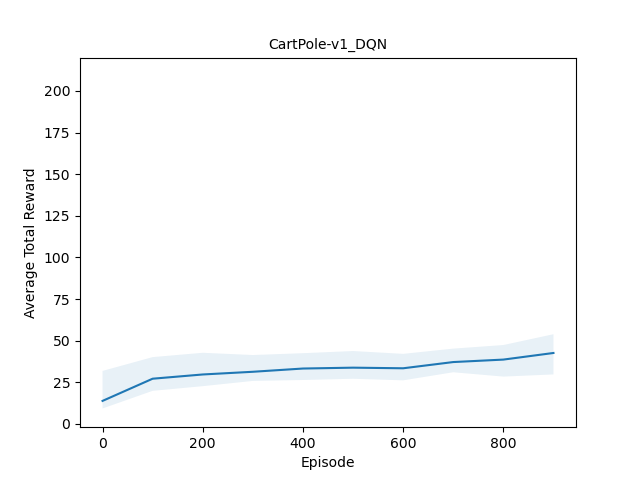
\includegraphics[width=0.6\textwidth]{graphs/CartPole-v1_DQN.png}
    \label{fig:dqn_cartpole}
% YOUR SOLUTION
\end{solution}


\newpage
\section*{Problem 2: Double DQN (21 pts)}

\subsection*{2.1: Double DQN plot (10 pts)}
\begin{solution}[height=9cm]
% TODO: Put your figures
    \centering
    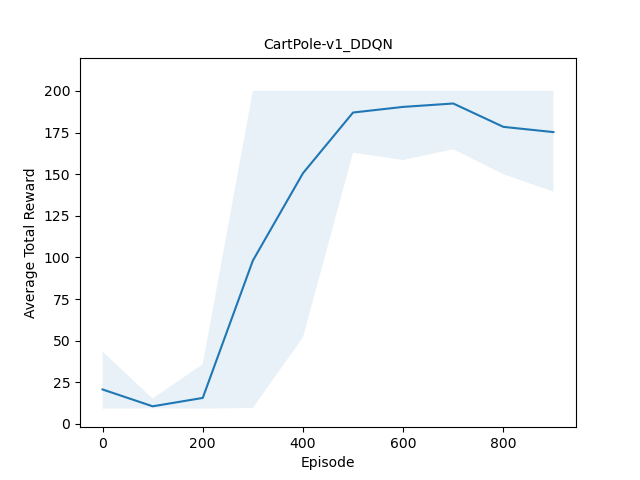
\includegraphics[width=0.6\textwidth]{graphs/CartPole-v1_DDQN.png}
    \label{fig:ddqn_cartpole}
\end{solution}

\subsection*{2.2 DQN vs. Policy Gradient Algorithms (5 pts)}
\begin{solution}[height=8cm]
% YOUR SOLUTION
The Double DQN outperforms the policy gradient algorithm we wrote in Assignment 1 because it benefits from stable and efficient value-based learning, utilizing experience replay and target networks. Policy gradient methods directly optimize the policy but suffer from high variance in gradient estimates and typically require more samples, making them slower to converge. Double DQN’s use of a target network and decoupling action selection and evaluation mitigates overestimation bias, further improving learning stability and performance.
\end{solution}

\subsection*{2.3 Pros and Cons of Policy gradient methods (6 pts)}
\begin{solution}[height=8cm]
% YOUR SOLUTION
Policy gradient methods like N-step A2C are better for continuous or high-dimensional action spaces where modeling a stochastic policy is advantageous. DQN is preferable for discrete action spaces. 
\end{solution}

\clearpage
\section*{Feedback}

\textbf{Feedback}: You can help the course staff improve the course for future semesters by providing feedback. You will receive a point of you provide actionable feedback. What was the most confusing part of this homework, and what would have made it less confusing?
\begin{solution}[height=4cm]

The graph\_agents function was somewhat harder to follow, making it difficult to understand how to implement correctly. The style used in Homework 1 was much easier to follow. I think bringing this over to Hw2 may be beneficial.

\end{solution}

\textbf{Collaboration}: Detail the work division amongst your group below.
\begin{solution}[height=4cm]
Worked on this Solo.
\end{solution}

\noindent\textbf{Time Spent}: How many hours did you spend working on this assignment? Your answer will not affect your grade. Please average your answer over all the members of your team.
\begin{solution}[height=4cm]
\begin{table}[H]
    \centering
    \begin{tabular}{r|c}
        Alone &  \hspace{3em} 8 %ANSWER HERE%
        \\ \hline
        With teammates & \hspace{3em} %ANSWER HERE%
        \\ \hline
        With other classmates & \hspace{3em} %ANSWER HERE%
        \\ \hline
        At office hours & \hspace{3em} %ANSWER HERE%
        \\ \hline
    \end{tabular}
\end{table}
\end{solution}


\end{document}
